% Chapter Template

\chapter{Analysis and Results - Passive Monitoring} % Main chapter title

\label{Chapter5} % Change X to a consecutive number; for referencing this chapter elsewhere, use \ref{ChapterX}

\lhead{Chapter 5. \emph{Analysis and Results - Part 1}} % Change X to a consecutive number; this is for the header on each page - perhaps a shortened title

\section{Analysis}
The final purpose of our system is to provide analysis about the main issues present on the infrastructure. The way we process here is quite simple:

\begin{enumerate}
\item Putting together the related information
\item Spotting the anomalies
\item Trying to understand the causes
\end{enumerate}
Like in any system, we had to define domains on which the monitoring tool will be able to work. One of the first steps of this thesis was to determine what were or could be the main issues on the UCL's network. It's here that we will use those results. Each of these problems will be a domain in which we will define what are the relevant data, how they can help us and how to react after having analyzed them. The purpose of this chapter is to present you these domains and the methodology used inside them. Each of them have their particular needs and their related techniques of analysis.

\section{WiFi}
\subsection{Users}
This section of the application offers some aggregated statistics about the users of the \emph{WiFi network}. The main goal is to get some analysis of the actual utilization of the wireless infrastructure. It's more a set of indicators to help the administrators to get a global view of his network. 
\subsubsection*{WiFi Protocol}
This graph display the repartition of the users among the available \texttt{802.11} standards (i.e. 802.11a, b, g, n). The reason for this analysis comes from an earlier policy enforced on the UCL network that forbids the use of the \texttt{802.11b} protocol. Users connecting with such low bandwidth standard force the \emph{access point} to transmitting longer and can in consequence prevent the others to achieve higher receiving speed. Our analysis was created to help the administrators in future considerations in the same domain. By profiling the habits of the users, we can define the impact of such decision. As the quality of the service is one of the main concern, deactivating the utilization of a standard used by most of the devices could have heavy consequences.
The statistics are based by default on the connections of the last three months. It's to ensure that devices no longer using the network doesn't affect the result and keep the analysis as up to date as possible.
\paragraph*{Source:} The data used come from \texttt{SNMP}. At each cycle gathering the information of the \emph{devices} associated with the \emph{access points}, we get the information thanks to the value available on the controller. All the descriptions of the OIB come from the Cisco OID Browser \footnote{http://tools.cisco.com/Support/SNMP/do/BrowseOID.do}.

\begin{tabular}{|r l|}
\hline
\textbf{Object} & \texttt{bsnMobileStationProtocol} \\
\textbf{Description} & \parbox{11cm}{The 802.11 protocol type of the client. The protocol is mobile when this client detail is seen on the anchor i.e it's mobility status is anchor.} \\
\textbf{OID} & 1.3.6.1.4.1.14179.2.1.4.1.25 \\
\textbf{MIB} & AIRESPACE-WIRELESS-MIB \\
\hline
\end{tabular}

\subsubsection*{SSID Utilization}
Here, we count the number of users by \texttt{SSID}. As before, the goal is to provide a profile of the users to the administrators. Such measures can help to adapt the policies related to each \texttt{VLAN} and defining the load of each of them. It could help to diagnostic a useless \texttt{VLAN} or in the opposite, allow to detect an overloaded one that could be caused by an improper use of the network. The supposed utilization and the actual one can be really different and such indicators can help to adapt the configurations.
\paragraph*{Source:} As before, we mainly aggregate the data available on the controller.

\begin{tabular}{|r l|}
\hline
\textbf{Object} & \texttt{bsnMobileStationSsid} \\
\textbf{Description} & \parbox{11cm}{The SSID Advertised by Mobile Station.} \\
\textbf{OID} & 1.3.6.1.4.1.14179.2.1.4.1.7 \\
\textbf{MIB} & AIRESPACE-WIRELESS-MIB \\
\hline
\end{tabular}

\subsection{Access Point}
This section group several analysis related to the \emph{access points}. In a network with several hundreds of \emph{access point}, it can be difficult to diagnostic and monitor each one of them. By centralizing and aggregating the data, we allow the network managers to save time by automatizing lot of computation. In this part of the application, we have access to the monitoring of each access point currently associated with the controller.

\subsubsection*{Load}
A fundamental piece of information related to an \emph{access point} is the load. We monitor each spot continuously and record its state several times per hour. By analysing those data, we are able to plot graphs representing the load throughout the days. We need two information: the \textit{quantity} of data transiting on the link and the \textit{maximum speed} of that link. Concretely, each \texttt{AP} own two bytes counters that are incremented each time a byte is received or sent. The other information required is the link speed connecting the spot. This information alone can be useful to diagnostic bandwidth issues. 
\paragraph*{Links} In a big network, it can be difficult to keep track of which links were updated and which ones were not. By collecting these data, we were able to find that two \emph{access points} were still connected with a \texttt{10 Mbits} link. In this case, the main cause was that those concerned devices were not managed by the SGSI and by consequence were not upgraded with the others. Those AP are in the \emph{Stevin} building.
This is the proof that even such simple data can help to diagnostic some inconsistency in the network.

\begin{figure}
   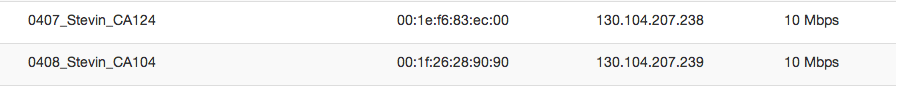
\includegraphics[width=\textwidth]{Pictures/chapter5/slowLinks.png}
   \caption{Example of 10Mbits Links (26/06/2014)}
\end{figure}

\paragraph*{Pattern of Utilization} By taking a look at the results, we can see during which periods of time the access point are the most active. In this example, we have taken a access point in the \emph{Leclercq} building and displayed the result of several days of monitoring. As expected, quite no activity is detected during the night and it only begins around 9 am. 

\begin{figure}
   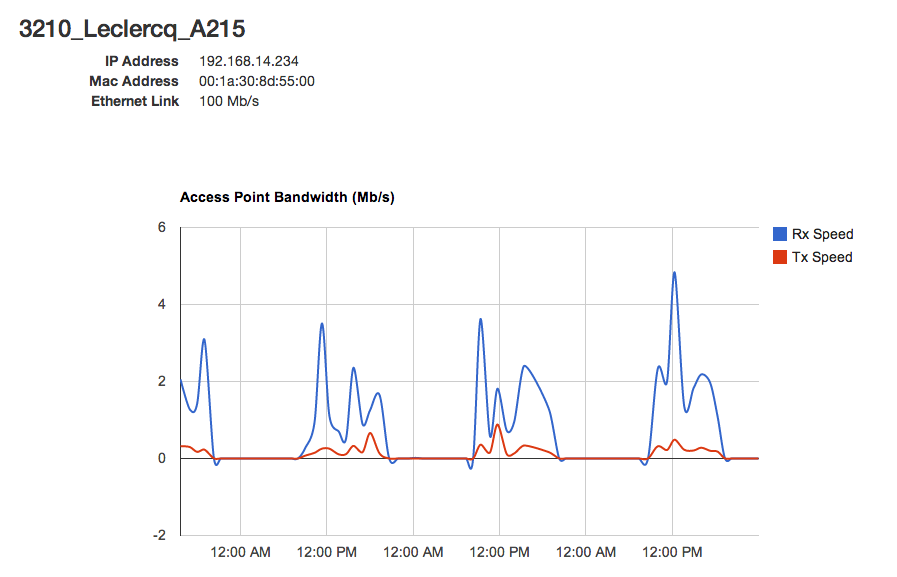
\includegraphics[width=\textwidth]{Pictures/chapter5/apLoad.png}
   \caption{Access Point Load}
\end{figure}

\paragraph*{Sources} Here again, we use the data available on the controller. The first data collected are the bytes counters of each \emph{access points}.

\begin{tabular}{|r l|}
\hline
\textbf{Object} & \texttt{cLApEthernetIfRxTotalBytes} \\
\textbf{Description} & \parbox{11cm}{This object represents the total number of bytes in the error-free packets received on the interface.} \\
\textbf{OID} & 1.3.6.1.4.1.9.9.513.1.2.2.1.13 \\
\textbf{MIB} & CISCO-LWAPP-AP-MIB \\
\hline
\end{tabular}

\begin{tabular}{|r l|}
\hline
\textbf{Object} & \texttt{cLApEthernetIfTxTotalBytes} \\
\textbf{Description} & \parbox{11cm}{This object represents the total number of bytes in the error-free packets transmitted on the interface.} \\
\textbf{OID} & 1.3.6.1.4.1.9.9.513.1.2.2.1.14 \\
\textbf{MIB} & CISCO-LWAPP-AP-MIB \\
\hline
\end{tabular}

The next step is to obtain the speed of each link connected to an \emph{access point}. This time again we use the \texttt{SNMP} protocol to get the information from the controller.

\begin{tabular}{|r l|}
\hline
\textbf{Object} & \texttt{cLApEthernetIfLinkSpeed} \\
\textbf{Description} & \parbox{11cm}{Speed of the interface in units of 1,000,000 bits per second.} \\
\textbf{OID} & 1.3.6.1.4.1.9.9.513.1.2.2.1.11 \\
\textbf{MIB} & CISCO-LWAPP-AP-MIB \\
\hline
\end{tabular} 

\subsubsection*{Interfaces}
Each \emph{access point} has two WiFi interfaces. The first one emits at \texttt{5Ghz} and the second at \texttt{2,4Ghz}. For each interface, the controller provides a lot of information that can be used in parallel of the previous ones. The first that we gather is the \textit{number of users} currently associated to the interface. We complete that piece of information with the quantity of users with a poor \texttt{Signal-Noise Ratio} (SNR). This analysis allows to diagnostic the efficiency of the access point. Even if it can be considered normal to have a couple of users in this category, if the proportion is constantly high, it can be an indicator that a supplementary \emph{access point} may be helpful or that the location of the AP is problematic. The problem have to be put in perspective with the RF environment (i.e \emph{Rogue Access Point} or physical walls) which is outside the scope of this system. 
Finally, we complete this analyse with a monitoring of the \emph{channel utilization}. A high utilization of the channel results in poor connection quality for the user and could indicates weak RF conditions.

\begin{figure}
   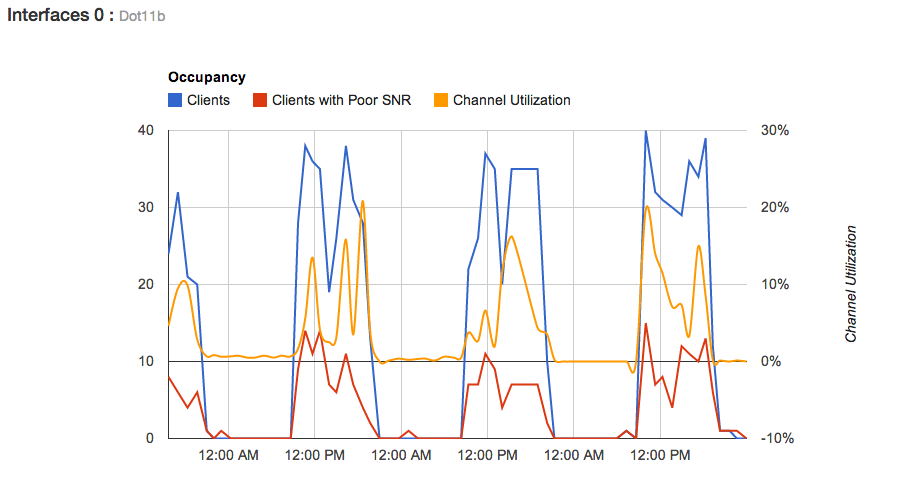
\includegraphics[width=\textwidth]{Pictures/chapter5/interfaceLoad.png}
   \caption{A 2,4GHz Interface}
\end{figure}

\paragraph*{Poor SNR} To illustrate our results, we have taken the 2,4GHz interface of the previous access point (i.e 3210 Leclercq A215) during the same period of time. As we can see, the load of the access point is correlated with the number of people connected to the interface. In this situation, we observe that there is an average of one-third or one-fourth of users with a poor SNR. This can be related to the configuration of the building. There is a large number of walls that separate the class room. The last thing to consider is the definition of a \emph{poor snr}. The value is defined by the controller and the number of clients with a weak signal is directly compute by it. In definitive, we do not have access and control on that parameter. Finally, to understand the importance of this result, we have to be aware that if a large portion of users have a low signal, it can influence the devices with a good one. In fact, the access point may have to spend more time to send data and by consequence is unavailable for the others connections.

\paragraph*{Channel Utilization} The channel is a shared resource and need to be available to be used. The utilization of the channel is an important indicator to the network administrators. It allows them to estimate the quality of the users connections. If the medium is used more than fifty percent, latency-sensitive applications can experience some performance issues\cite{ciscoVowlan}. A continuous monitoring of that value can help to detect and diagnostic such related problems. In our example, we can see that there is some maximum peaks at twenty percent of utilization which is totally acceptable. 


\paragraph*{Sources} The controller keeps entries for each \emph{interface} of each access point. We gather and cross all these data to generate some logs about each \emph{access point} and all the related \emph{interfaces}.

\begin{tabular}{|r l|}
\hline
\textbf{Object} & \texttt{bsnAPIfLoadNumOfClients} \\
\textbf{Description} & \parbox{11cm}{This is the number of clients attached to this Airespace AP at the last measurement interval.} \\
\textbf{OID} & 1.3.6.1.4.1.14179.2.2.13.1.4 \\
\textbf{MIB} & AIRESPACE-WIRELESS-MIB \\
\hline
\end{tabular}

\begin{tabular}{|r l|}
\hline
\textbf{Object} & \texttt{bsnAPIfPoorSNRClients} \\
\textbf{Description} & \parbox{11cm}{This is the number of clients with poor SNR attached to this Airespace AP at the last measurement interval.} \\
\textbf{OID} & 1.3.6.1.4.1.14179.2.2.13.1.24 \\
\textbf{MIB} & AIRESPACE-WIRELESS-MIB \\
\hline
\end{tabular}

\begin{tabular}{|r l|}
\hline
\textbf{Object} & \texttt{bsnAPIfLoadChannelUtilization} \\
\textbf{Description} & \parbox{11cm}{Channel Utilization.} \\
\textbf{OID} & 1.3.6.1.4.1.14179.2.2.13.1.3 \\
\textbf{MIB} & AIRESPACE-WIRELESS-MIB \\
\hline
\end{tabular}



\subsection{Rogue Access Points}

\section{Controller}
The controller logs are divided in several categories. Each of them defined a list of log related to that category. The main idea here is to analyse the activity of each domain of logs and trying to spot irregularities. We make the hypothesis that when something went wrong, the related category will emit a larger number of logs. By monitoring that activity, we will be able to identified in which part of the infrastructure the issue happened.

\subsection{Components Activity}


\section{DHCP}
These analyses aim to detect \emph{DHCP} related issues. The allocation  of IP addresses is a fundamentals component in our network. Being able to detect when problems appears and advertise them could help to make a quicker and more efficient response.

\subsection{Leases}
The main problem with a DHCP is the allocation of ranges of addresses. It's always difficult to determine the quantity of required IP by VLAN. Moreover, when such problems arise, it can be hard to be aware of them. Most of the time, users don't report the problem and when they do, their descriptions state only that they can't connect which is not very useful. Being able to automatically detect a lack of IP addresses can be very time saving for any administrators. Even is such information are available in the \emph{DHCP} logs and that the servers could send warnings, centralizing these information aside data related to all the other components of the infrastructure can lead to more powerful analysis. 

\subsection{Crash}


\section{Radius}


\subsection{Authentication Success Rate}




